\chapter{State of the art}

Cloud storage services have been steadily increasing in popularity and reached mainstream status in the past decade. In essence, these services allow users to upload and store files on the internet without the need to own the physical storage medium. Files can be accesed from almost any devices with an internet connection, provided that the user follows the required authentication process.

Most cloud storage services provide free plans, which usually limit the total storage capacity. Their premium plans either follow the subscription business model or even go as far as to require a one-time purchase in exchange for a lifetime subscription.

As of \monthyeardate\today, some of the most popular\footnote{\url{https://www.zdnet.com/article/google-plans-to-leverage-g-drive-for-broader-enterprise-footprint-team-management-and-collaboration/}} names ring a bell even to non-technical users:
\begin{itemize}
\item Microsoft OneDrive
\item Google Drive (800 million active users, March 2017)
\item Apple iCloud Drive
\item Box
\item Dropbox
\end{itemize}

This is no coincidence. Many tech companies attempt to draw users into their own ecosystem, especially when it is a vast one. Consumers that already use several products owned by the same company tend to favor that company's other products over their direct competitors. There are multiple advantages in doing so. For one, familiarity is a key factor. A competitor's service may be more difficult to use by a consumer who is unfamiliar with it. On top of that, a single ecosystem provides greater cohesion between its elements. This translates into better integration between services, which improves the overall experience.

Two of the largest technology companies -- \mbox{Apple Inc.} and \mbox{Alphabet Inc.} -- are commonplace examples of this strategy. Users who sign up for a free Gmail account automatically receive an associated \mbox{15 GB} storage plan on Google Drive. Moreover, this storage is shared among three different services: Google Drive, Gmail and Google Photos. Similarly, Apple offers \mbox{5 GB} of free storage on iCloud:

\begin{quote}
iCloud is built into every Apple device. That means all your stuff — photos, files, notes, and more — is safe, up to date, and available wherever you are. And it works automatically, so all you have to do is keep doing what you love. Everyone gets \mbox{5 GB} of free iCloud storage to start, and it’s easy to add more at any time.
\end{quote}

It seems that offering free storage is similar in concept to planting a seed that will reap a greater harvest. Indeed, making a user familiar with your service will make him more likely choose your premium plan when deciding to upgrade, instead of your competitor's.


\section{User Interface}

File hosting services usually allow access via \mbox{HTTP}, with some of them also supporting \mbox{FTP}. As a consequence, the main way of interacting with them is via a web platform.

\begin{figure}[h]
\caption{Web interface of the Dropbox file hosting service}
\centering
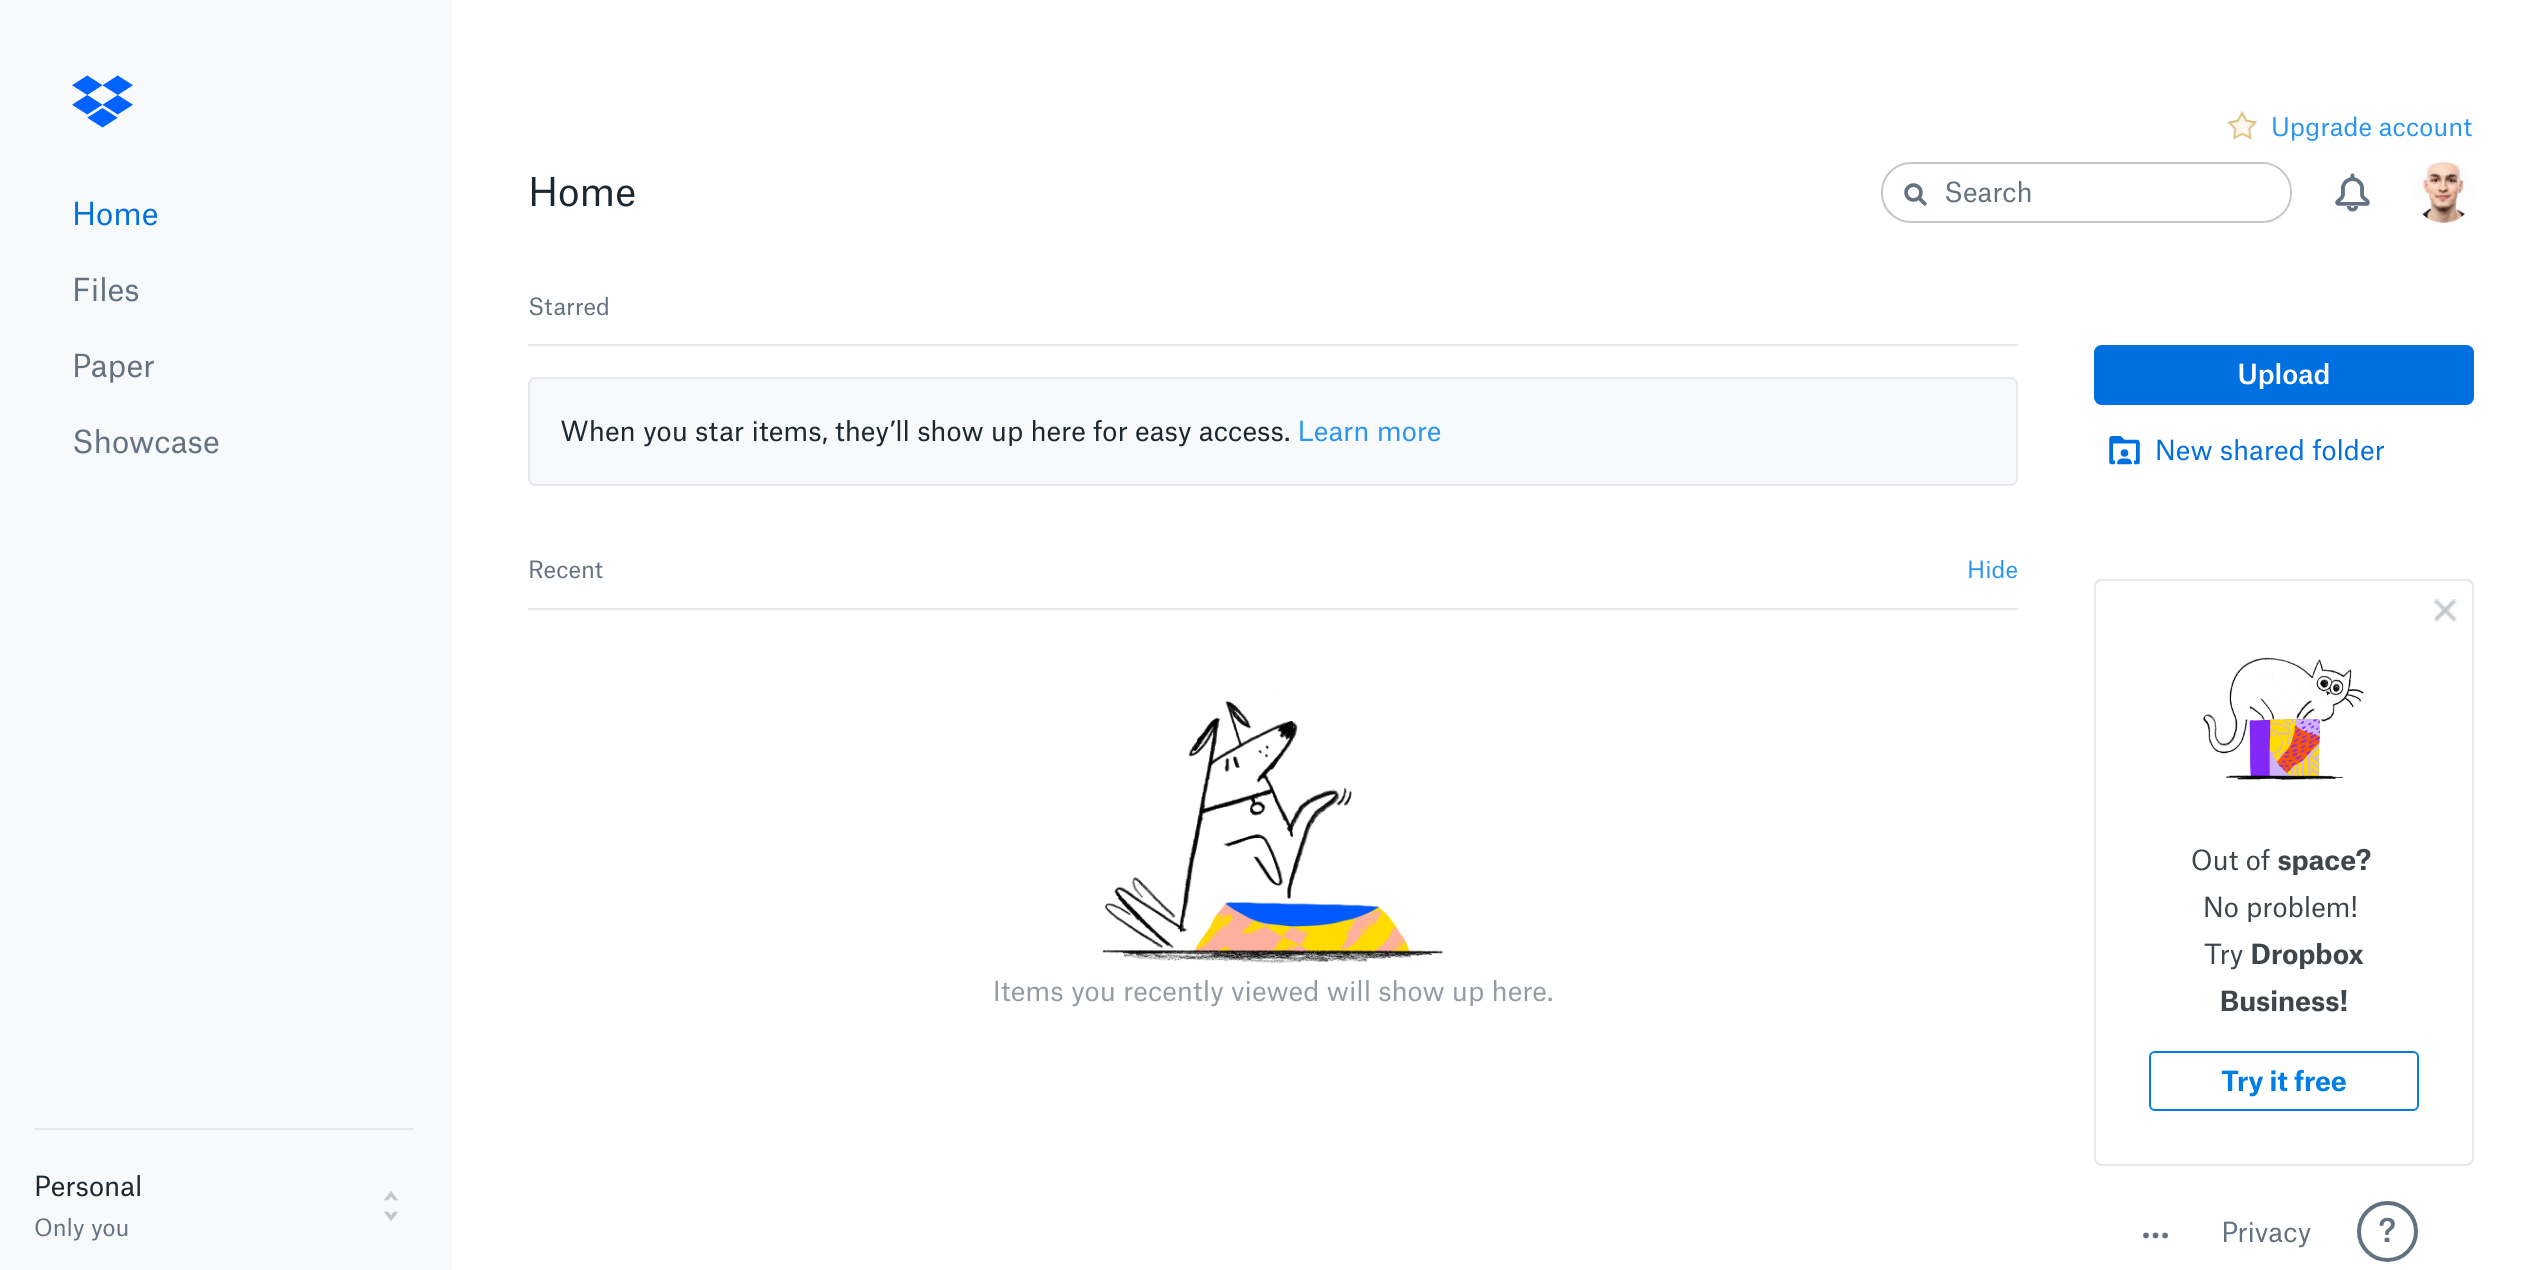
\includegraphics[width=\textwidth]{dropbox_homepage}
\end{figure}

\section {Main advantages}

\section {Main disadvantages}

